

% -------------------------------------------
\section{Introduction}


\subsection{What is MARS?}
MARS is a new network services and workflow system that supports structural network analyses and generalized network dynamics analyses. It is accessible through the internet and can serve multiple simultaneous users and software applications. In addition to managing various types of digital objects including networked data, MARS
provides services that enable applications (and UIs) to add, interrogate, query, analyze, and process data.

\begin{figure}[H]
\centering
%\label{fig:ebola-kshell-not-effective}
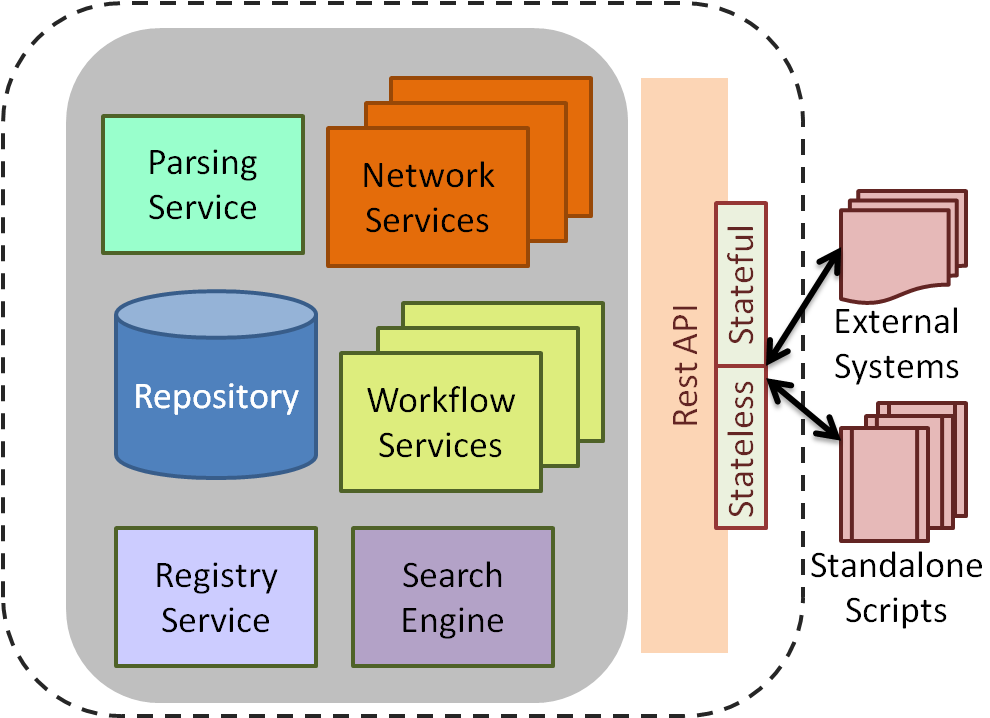
\includegraphics[trim = 0.0in 0.0in 0.0in 0.0in,scale=0.4]{mars-overall}
\caption{
Overview of the MARS system.
}   %   
\label{fig:mars-overall}
\end{figure}

\subsection{Features}

\begin{itemize}
\item Modular, interoperable categories
of services, where each service can be a distinct, relocatable process.
\item Stateless (REST-ful) and stateful (using session management) API.
\item SQL-like query grammar with special features for network dynamics.
\item Built-in search engine, for quey grouping, sharing and retrieval.
\item Database for storing networked data along with metadata.
\item \textbf{New in v2.0} Distributed architecture, multiple services run separately  on different VMs. Services communicate using HTTP requests.
\item \textbf{New in v2.0} Workflow service to execute a set of user-defined steps for analyzing networked data.
\item \textbf{New in v2.0} Data plotting service. Integrated within the workflow service. Currently, is using matplotlib but can be extended to other 3rd party plotting tools (e.g. ggplot, D3).
\item \textbf{New in v2.0} Network Measure service with a dedicated broker. The measure service has to be running on shadowfax.
\item \textbf{New in v2.0} Extended database schema.



\end{itemize}



